\subsection{Tune measurements}

In the combiner ring the beam does a maximum of 4 turns. 
This makes the situation fundamentally different from a storage ring or 
synchrotron where particles make millions of turns so avoiding the integer or 
half integer resonances are not of the same importance. 
However, tune measurements can give detailed information about the optics and 
possible errors in the machine or in the model.

For the tune measurement the machine was set up for multi turn by shifting 
the timing of the extraction kicker to a later point in time. 
In order to measure the tune the beam was injected 
off the closed orbit into the combiner ring. 
The focusing strength of a quadrupole was changed to observe 
if the changes could be predicted by the model. 
The ideal situation would have been to change quadrupole by 
quadrupole and measure the change in tune.
However, in order to get an accurate tune measurement 
we can only tolerate small beam losses and 
this limits the amount of different settings that could be used.


To measure the tune the following steps have been done. 
They are described in detail in the forthcoming sections.
\begin{enumerate}
\item
Set up the combiner ring so the beam is circulating for at least 60 turns 
without losses.
\item
Acquisition of the signals from the BPMs with different settings of the magnets.
\item
Calculate the beam position for every BPM and every turn.
\item
Determine the average position over several pulses.
\item
Compensate for the charging-up effect.
\item
Fit each signal with a sinusoidal curve.
\item
If the fit is good enough, save the value and put it in the histogram with 
the other BPMs from the same measurement.
\item
Compare the values to the model.
\end{enumerate}


 
Figure~\ref{fig:bpm_not_charging_up} shows typical traces from a BPM directly read out 
from the control system. In the top the current trace is displayed, 
in the middle the horizontal position and in the bottom the vertical position. 
Every dip marks one turn in the combiner ring. 

Only the 12 first turns could be used due to strong dechoherence 
of the oscillation. The oscillation is damped to the closed orbit for the ring. 
Since the beam normally only does 4 turns in the combiner ring 
the closed orbit is not well-determined. 
\begin{figure}[!h]
\centering
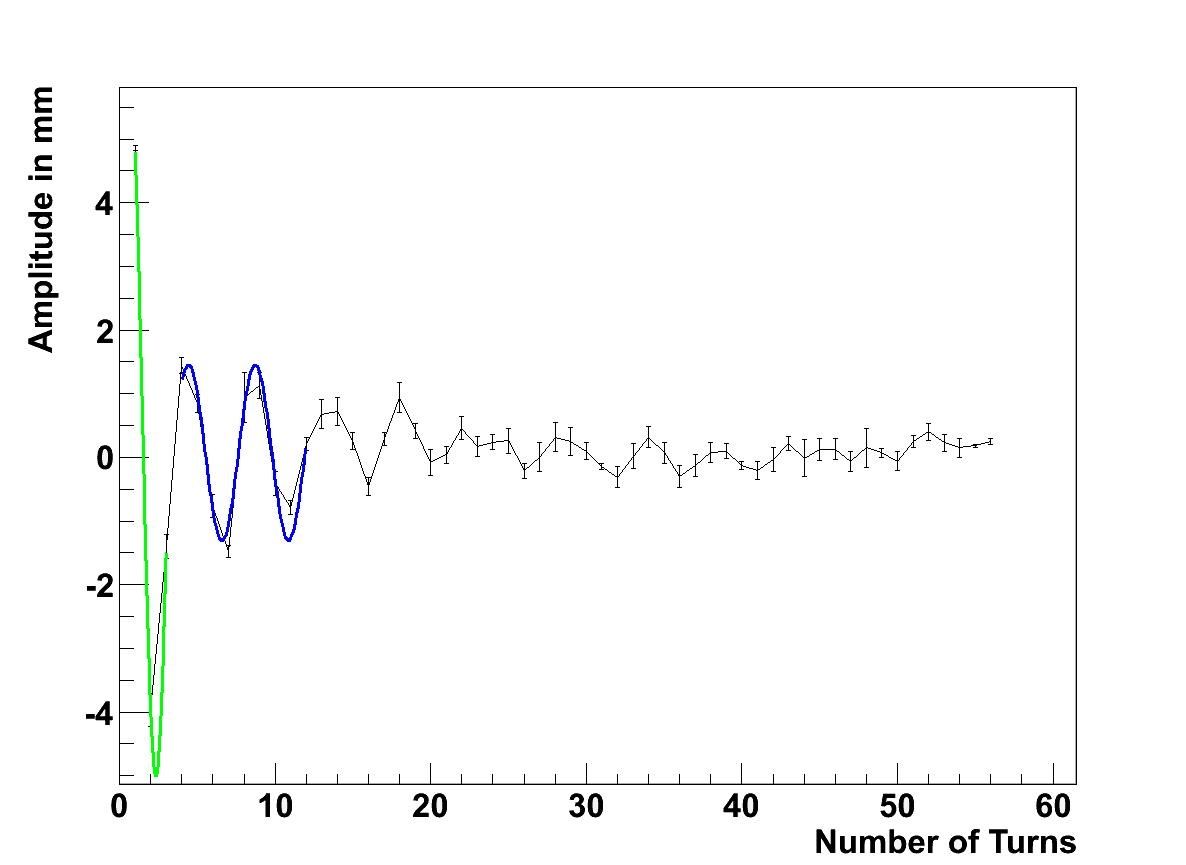
\includegraphics[width=0.66\linewidth]{fit_BPM8.png}
\caption{A sinusoidal fit over the position for different turns. \label{fig:fitOfPosition}}
\end{figure}
All fits were checked manually and if seen to fit the signal they were accepted and
placed as a count in a histogram. 
The histogram was then fitted with a Gaussian function and the mean and 
the $\sigma$ were saved for each measurement.
The fact that the tune or period of a sine is 
independent of amplitude of the oscillation makes the tune measurement 
independent of absolute calibration errors in the BPMs.
 
In order to determine if measure values are above or below 0.5, 
a quadrupole is changed by a few percent. 
Depending on if the quadrupole is focusing or 
defocusing in that plane and if the tune goes up or down it is possible to 
determine if the tune is above or below 0.5.  

The number in the table corresponds to the number on the x-axis in 
Figure~\ref{fig:tuneModelVsMeasure}.
It seems that the model slightly overestimates 
the change in tune when varying the focusing of a quadrupole.
Because of the large uncertainty of the measurement 
it was not possible to conclude that there was any error in the model.

\begin{figure}[!h]
\centering
\subfloat[]{
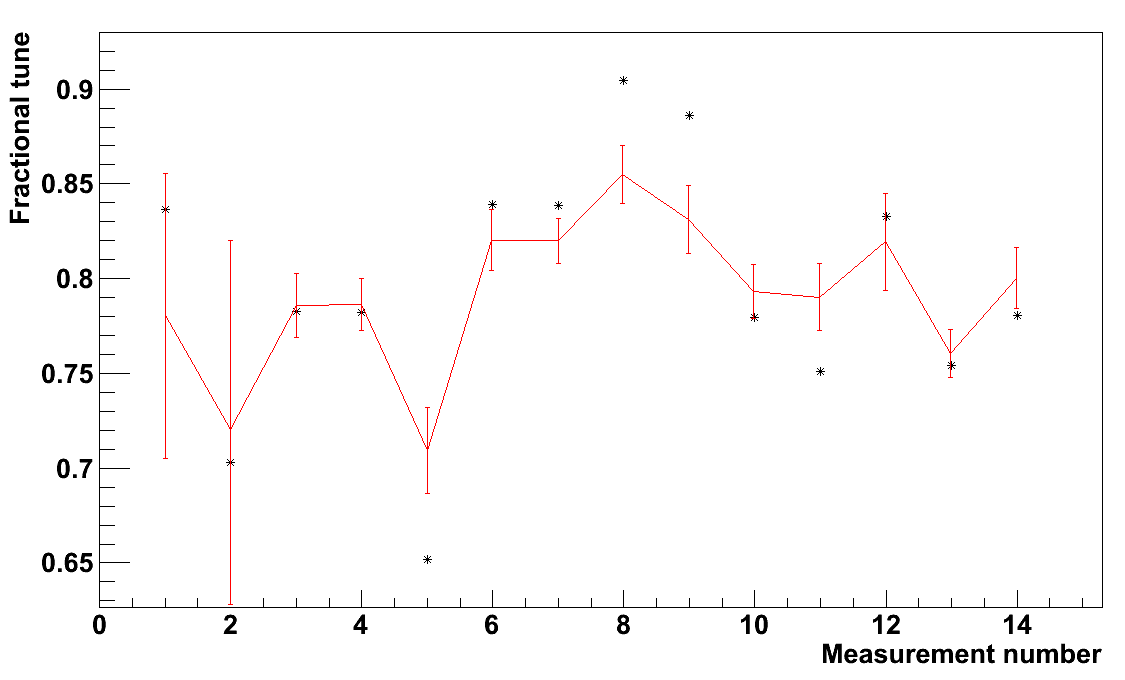
\includegraphics[width=0.48\linewidth]{horizontal_tuneVsModel.png}
\label{fig:tuneModelVsMeasureHorizontal}
}
\subfloat[]{
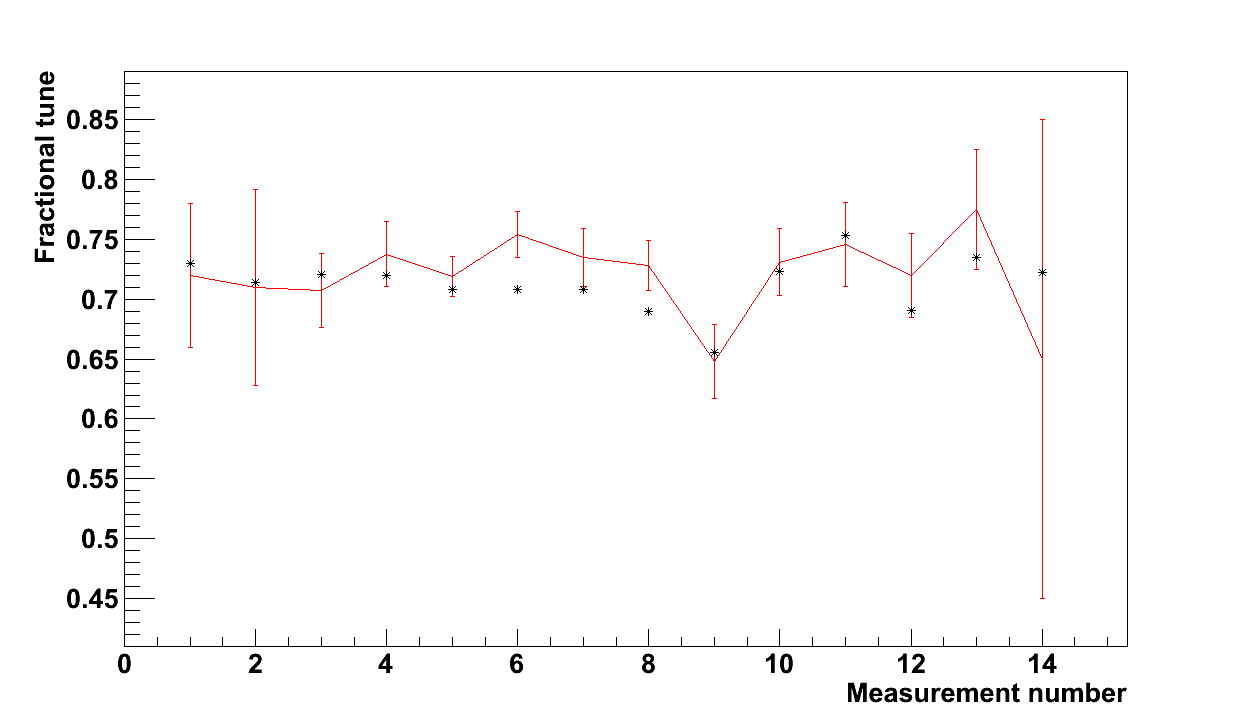
\includegraphics[width=0.48\linewidth]{vertical_tuneVsModel.png}
\label{fig:tuneModelVsMeasureVertical}
}
\caption{Example tune measurement when different quadrupole circuits where modified (red error bars)
compared to the model expectations (marked as *).
\label{fig:tuneModelVsMeasure}
}
\end{figure}
 

The fit also provided information about the phase at each BPM. 
In this case the tune for the fit was fixed to a value obtained in the previous section 
while phases were allowed to vary. 
The phase is aliased but by forcing the fit to be between $0 - \pi$ 
it is possible to compare the phases between different pickups. 
The difference in phase between two successive pickups were added together 
to get the overall phase advance. 
Figure \ref{fig:phaseAdvHorizontal} shows the phase advance for 
the horizontal plane while figure \ref{fig:phaseAdvVertical} shows it 
for the vertical plane. The error bar is 1 $\sigma$ and 
is calculated using the fitting environment in ROOT which takes the error bar into account
when calculating the uncertainty in each parameter.
 
\begin{figure}[!h]
\centering
\subfloat[]{
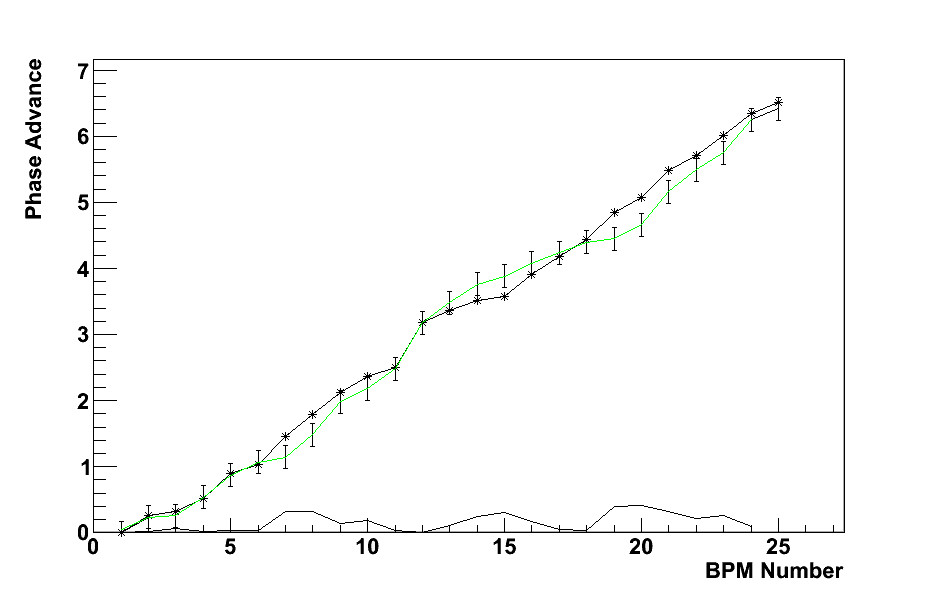
\includegraphics[width=0.48\linewidth]{phaseAdvHorizontal.png}
\label{fig:phaseAdvHorizontal}
}
\subfloat[]{
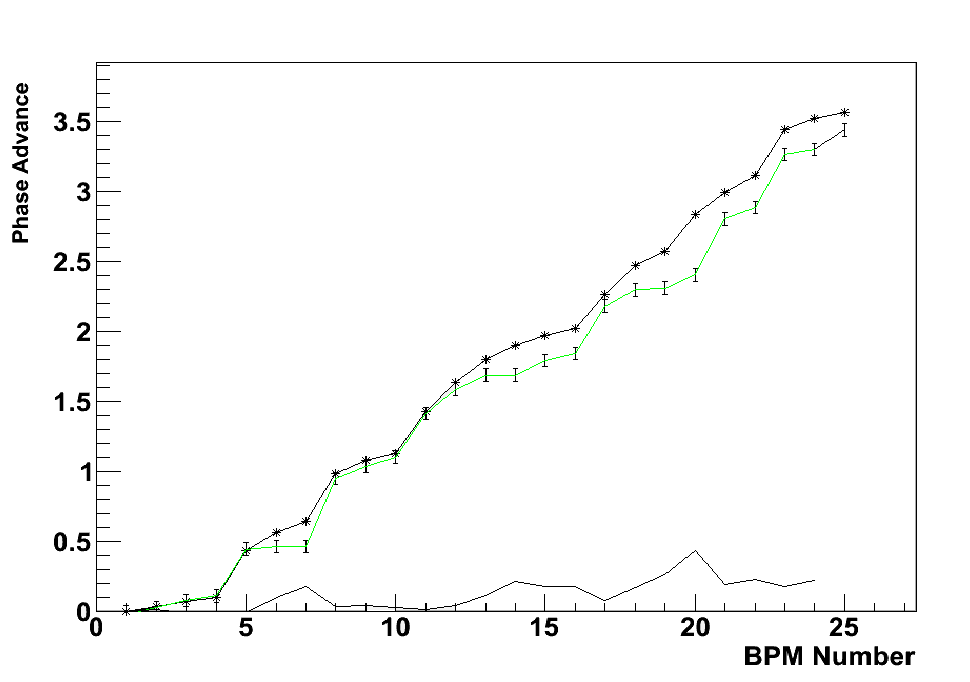
\includegraphics[width=0.48\linewidth]{phaseAdvVertical.png}
\label{fig:phaseAdvVertical}
}
\caption[Phase advance]
{Comparison between the model, marked as *, 
and the measurement represented with the green error bars.
Left is horizontal plane and right is vertical one.
The black line shows the absolute difference between the measurement 
and the model. \label{fig:phaseAdv}}
\end{figure}
 

The result is in overall agreement with the model. 
Although, the precision needed to establish if there is a discrepancy 
between the measurement and the model between two consecutive pickups was not achieved. 
However, it provides the additional information that we are close to the design tune. 
In order to make more precise measurements it was important 
to have more turns before the oscillation decohere by reducing the chromaticities.
The best result obtained for the vertical oscillation is shown in 
Figure~\ref{fig:tune:sextopole_vertical}. 
However, the use of sextupoles introduces extra complexity
because they change the optics and tune due to feed-down.

\begin{figure}[!h]
\centering
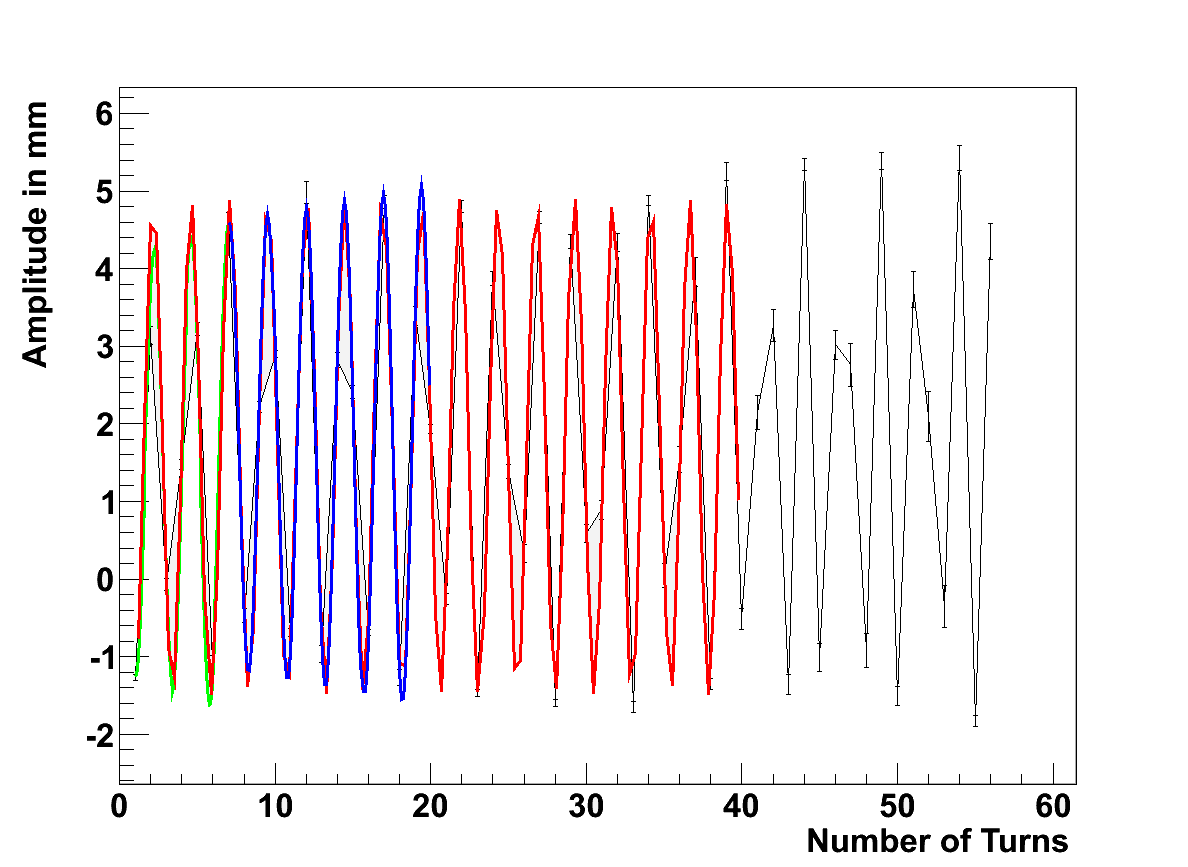
\includegraphics[width=0.45\linewidth]{sextopole_vertical.png}
\caption{Vertical oscillation with reduced chromaticity.  \label{fig:tune:sextopole_vertical}}
\end{figure}
 
The overall agreement between the tune measurements and 
the model indicates that there are no major errors in the model. 
In order to reach higher accuracy it would be necessary to implement 
an achromatic optics with reduced chromaticity.
 
